\documentclass[twocolumn, a4paper]{ieicejsp}
\usepackage[english]{babel}

\usepackage{graphicx}
\usepackage{amsmath}
\usepackage{amssymb}
\usepackage{amsthm}
\usepackage{epsfig}
\usepackage{listings, color}
\usepackage{url}

\title{{\bf On assesing Provider mobility in ICN networks}}
\author{
    Jairo Eduardo L\'{o}pez$^1$ \\ \and
    Takuro Sato$^1$ 
}
\affliate{Graduate School of Information and Telecommunications Studies, Waseda University$^1$}

\begin{document}
\maketitle
%\twocolumn[
%\centerline{\huge \bf On Provider mobility in ICN networks}
%\medskip
%\centerline{Jairo Eduardo L\'{o}pez$^{1}$, Takuro Sato$^{2*}$}
%\medskip
%\centerline{${}^{1,2}$ Graduate School of Information and Telecommunications
%Studies, Waseda University}
%\centerline{jairo at ruri dot waseda dot jp${}^{1}$, t-sato at waseda dot jp${}^{2}$, ${}^{*}$Fellow, IEEE}
%\bigskip
%]

\section{Abstract}
%It has been known for some time that our current Internet infrastructure
%requires an overhaul. Over the last 3 decades there have been attempts to solve
%the main issues plaguing our current network infrastructure. A lot of the 
%issues have been solved in ad-hoc ways, while others have been completely
%ignored. Mobility, for example, has required the implementation of complex
%architectures which have patched the problem, but not solved it due to the 
%flat naming of our current network infrastructure. 

%Among the new ideas for a clean-slate network architecture, one of the most
%prominent has been Information Centric Networking (ICN), which takes content
%as the primary source of network traffic. This architecture shows a lot of
%promise and supports mobility out of the box. 

Information Centric Networking (ICN) is a clean-slate network architecture that
shows a lot of promise in supporting network mobility out of the box.  Due to
the number of different ICN proposals evaluating network architecture decisions
regarding mobility is not as easy as it should be.

This paper proposes a simple network topology and metric to assess ICN mobility,
having a mobile node travelling through a set path of points of attachment
(PoAs) to a network where another set of client nodes are located, using ns-3
and ndnSIM. We use our proposed mobility scenario to futher discuss improvements
in ICN mobility, specifically provider mobility.

\section{Introduction}
ICN, initially proposed by Van Jacobson, attempts to make content and not hosts,
the network's first class citizens \cite{Jacobson:2009:NNC:1658939.1658941}.
%This shift is well founded in fact \cite{cisco:2014:Online}
%\cite{ciscomobile:2014:Online}, meaning that any future network architecture
%should be able to handle high content demand and mobility.
 
%This particular shift to a
%content-oriented model is well founded in fact as most network analysis shows
%that for 2013 about 66\% of all IP traffic was caused by video transmission
%. Estimates put IP video tranmission at 79\% for 2018 
%\cite{cisco:2014:Online}.
%Another fact that makes this architecture compelling is that mobile IP traffic
%is currently at 3\% of the total IP traffic, but is estimated to increase 4
%fold in 5 years. 
%While still a smaller chunk of total IP traffic, about 53\% of current mobile
%IP traffic is video and is also expected to increase in the following years
%\cite{ciscomobile:2014:Online}. Taking these facts into account, it would seem
%beneficial for any future network architecture to take the high demand for
%content and mobility trend into account.

The ICN architecture is still under heavy debate, meaning that there are a lot
of competing proposals. 
%The variations between some proposals can be really subtle. 
The basic ICN architecture description and the most important ICN architecture
proposals have been summarized in \cite{6563278}. 

\section{Current status of mobility in ICN Approaches}

%In the basic ICN architecture, data can only be transmitted after a device has
%sent a request, i.e an Interest packet. For mobility, this means that when a
%mobile terminal changes its point of the attachment, the desired Interest
%packets have to be retransmitted \cite{Jacobson:2009:NNC:1658939.1658941}. This
%simple architecture structure, makes mobility, at least for the client, reliable.
%A prominent example is the CCNx proposal which is able to handle up to 97\% of
%requests under high mobility \cite{5698270}. 

In the case of producer/provider mobility, i.e when the content desired by
clients on the network is mobile and changing PoA, the results for ICN are
inconclusive \cite{Tyson:2012:SMI:2248361.2248363}. With ICN, there is a 
desire to reduce network complexity, however, most of the proposals to enchance
mobility scenarios require a reimplementation of the network architecture's
naming and addressing, tending to loosely follow the guide lines
established by Saltzer \cite{saltzer:namingandbindingnetworks} and further
commented on by Day \cite{Day:2008:PNA:1349793}. Before adding more complexity
to the network, we would like to know the status of provider mobility in a network
architecture with only the basic ICN attributes. In other to provide verifiable
answers, we have created a simple network topology and chosen some metrics to
better assess different proposals. For this paper we will compare simple ICN 
forwarding strategies. Our code base is available to all via Github at
\cite{githubndnmobi}.

%Some of the latest proposals using these methods
%can be found in \cite{6459937} \cite{6799694} \cite{DAC:DAC2752} \cite{6364701}
%\cite{6726304}.
%These proposals have their merits. 

\section{Implementation}
\label{sec:implementation}
We chose to obtain our metrics for a provider mobility scenario in ICN. We use 
ndnSIM \cite{ndn367}, an implementation of NSF's NDN \cite{nsfndn:2014:Online},
that uses the ns-3 network simulator \cite{ns3:2014:Online}. Our proposed 
topology is inspired by the cellular network topology of LTE \cite{sesia2011lte} and
is a simplication of it. In our topology, shown in figure \ref{fig:exptop}, there
is one mobile node constantly providing content via its wireless interface. The
mobile node changes it's PoA, while moving, when it is perpendicular to one of
the next 6 wireless ICN routers. Each two wireless ICN routers have Content
Stores with LRU policies and are connected by PtP connections. Both are also
connected with a third ICN router, using the same settings, that connects via a
CSMA/CD connections with 4 client nodes. This layout is repeated 3 times horizontally. 

\begin{figure}[h]
\centering
%\resizebox{\columnwidth}{!}{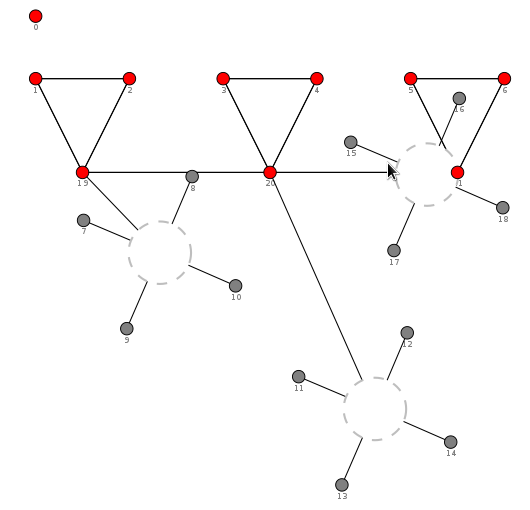
\includegraphics[scale=0.4]{topology.png}}
%\resizebox{0.65\columnwidth}{!}{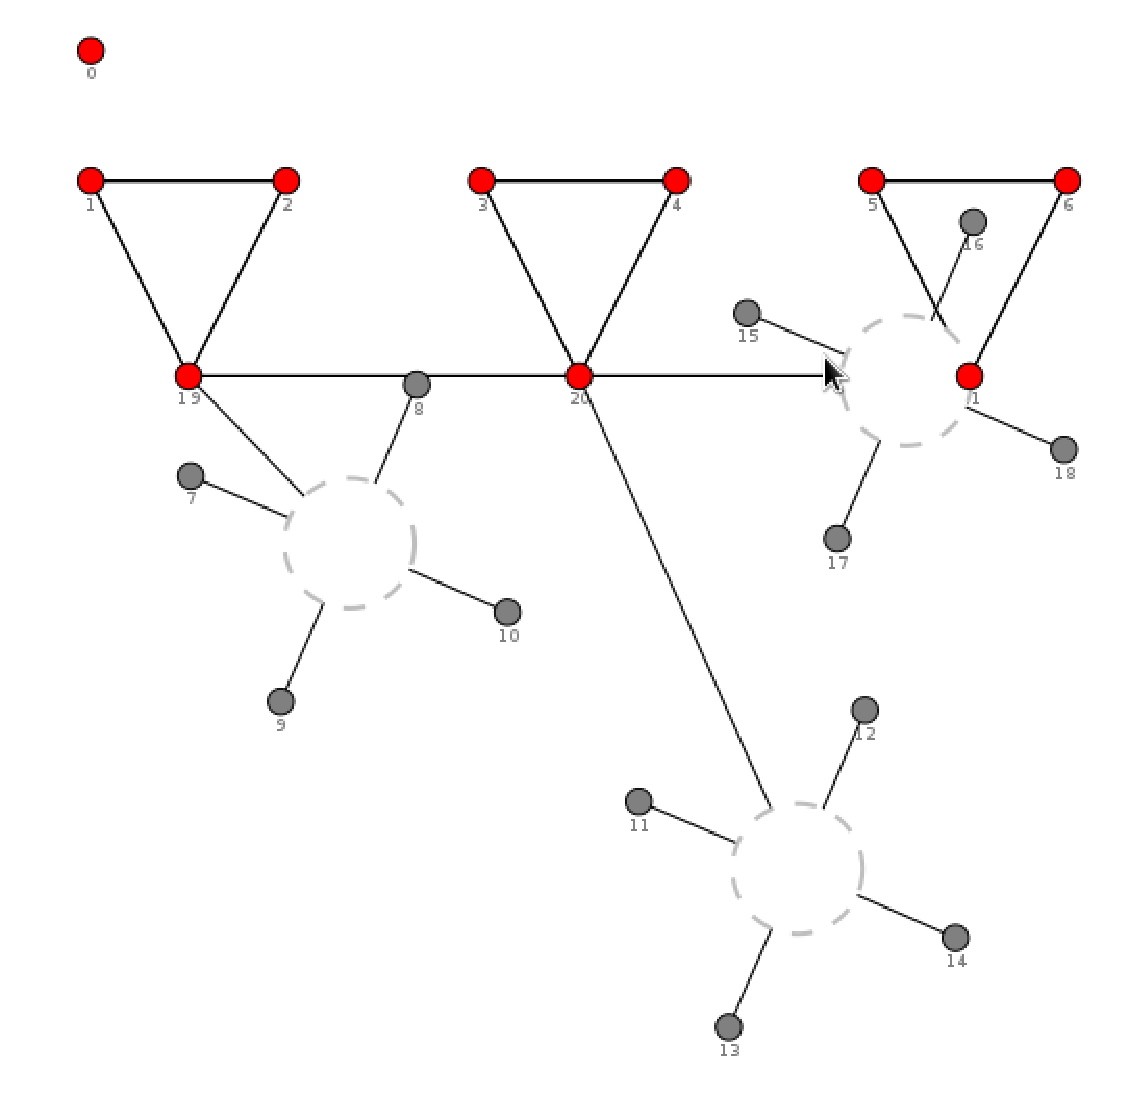
\epsfig{file=topology.eps}}
\resizebox{\columnwidth}{!}{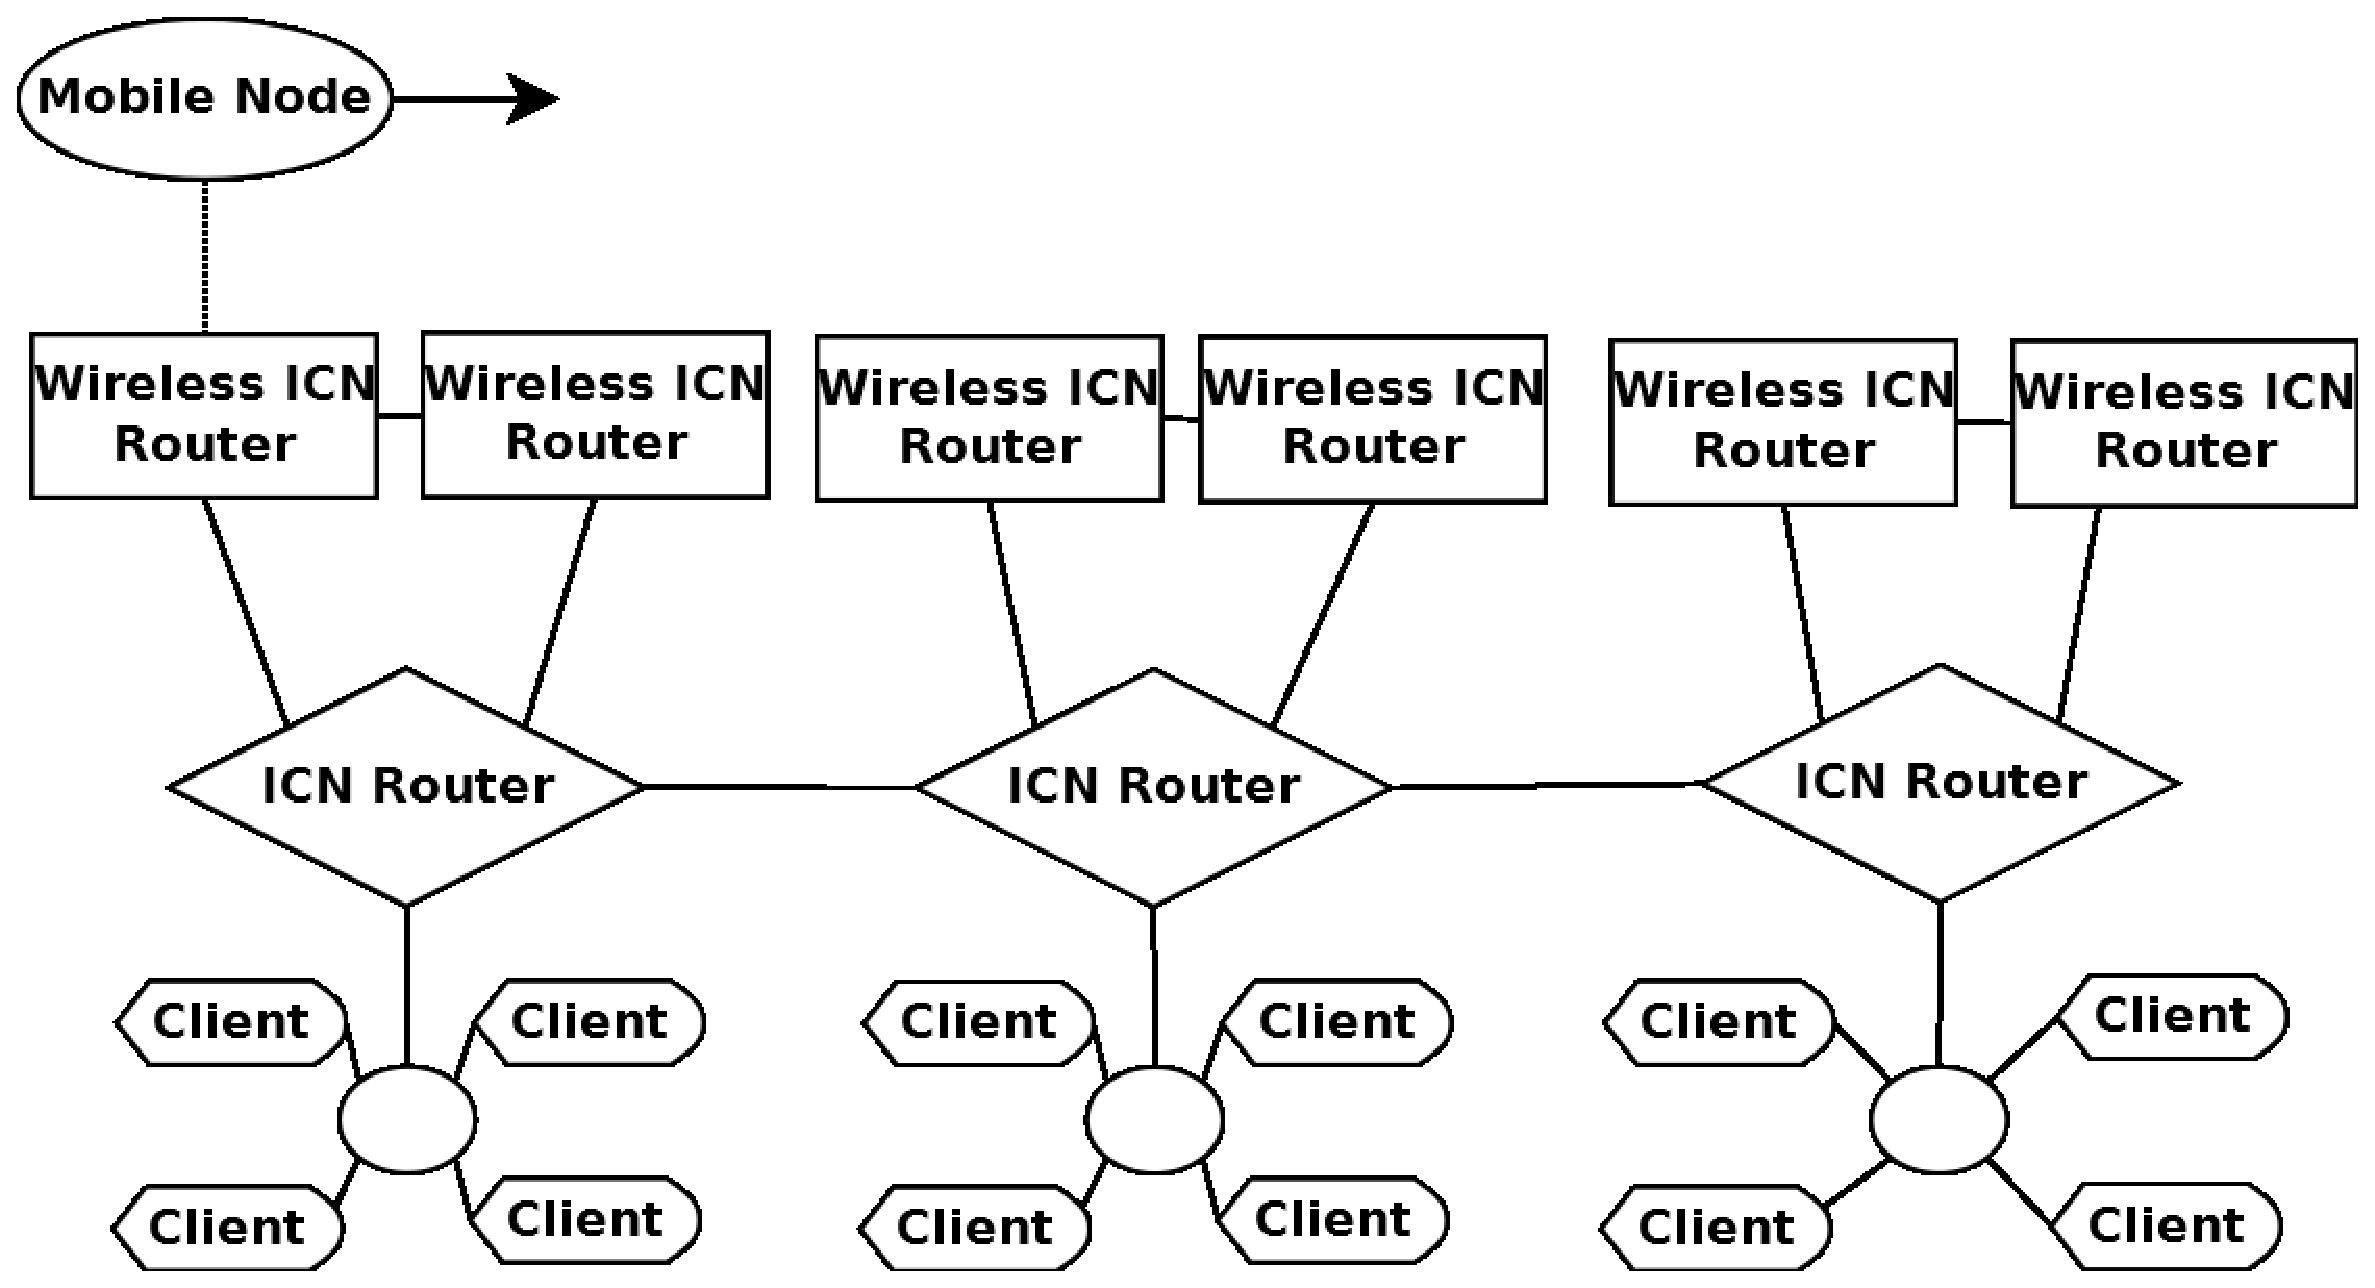
\epsfig{file=experiment.eps}}
\caption{Topology for experiments}
\label{fig:exptop}
\end{figure}

\section{Methodology}
To test the success rate of a ICN we measure the Satisfied Interest packets,
Interest packets that were transmitted and received the corresponding data, and
the Timed Out Interest packets, Interest Packets that were transmitted but
received no data and thus timed out. We also calculate the last sequence number
received by our NDN application to be able to compare the success rate for 
forwarding strategies. We ran the simulations on the topology described in
section \ref{sec:implementation}, changing only the forwarding strategy for
the ICN network. For this particular experiment, we chose the forwarding
strategies that include no network feedback and no naming/addressing resolution 
in order to assess provider side mobility in a basic ICN architecture. The
chosen strategies were Flooding, BestRoute and SmartFloooding strategies
\cite{ndn367}. All strategies had token bucket queues that limit the use of
ICN router interfaces when a certain number of Interest packets have been
transmitted and have not been satisfied. We also executed an idealized
simulation, where there is no mobility, on the same topology to be able to
judge the number of packets used to obtain the desired information. The clients 
generating the Interest packets were chosen randomly from the CSMA/CD connected
clients.

We executed the simulations a total of 10 times for each selected strategy.

\section{Results and Discussion}
%The results of our experiments can be seen in table \ref{tab:packetsum}. 
%Figure \ref{fig:sattimeint} shows the behavior of the network over time.

\begin{table}[h]
\centering
\resizebox{0.8\columnwidth}{!}{
\begin{tabular}[t]{|p{1.5cm}|c|c|c|c|c|}
\hline
 & Flooding & BestRoute & SmartFlooding & Ideal \\
\hline
Satisfied Interests & 5190.822 & 1840 & 5641.812 & 1289 \\
\hline
Timed Out Interests & 10130.679 & 4887 & 9719.665 & 0 \\
\hline
Total content received & 78.8 & 44 & 108.5 & 214 \\
\hline
$\sigma$ Total content received & 22.28 & 8.56 & 13.26 & 0 \\
\hline
Hop Count & 7.76 & 6 & 7.56 & 6 \\
\hline
$\sigma$ Hop Count & 1.43 & 0 & 1.48 & 0 \\
\hline
\end{tabular}
}
\caption{Averaged simulation results}
\label{tab:packetsum}
\end{table}

%\begin{figure}[h]
%\centering
%\resizebox{\columnwidth}{!}{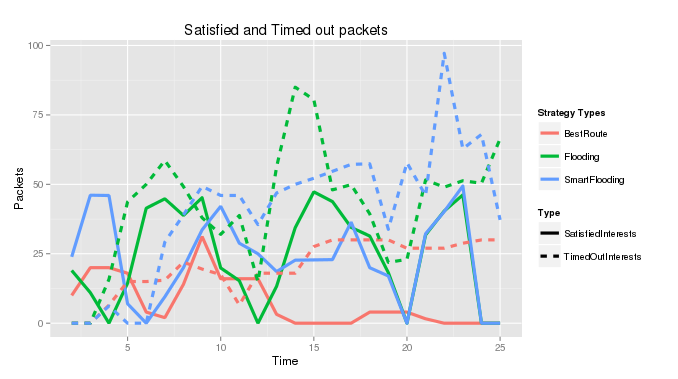
\includegraphics{satisfied-timeout.png}}
%\resizebox{\columnwidth}{!}{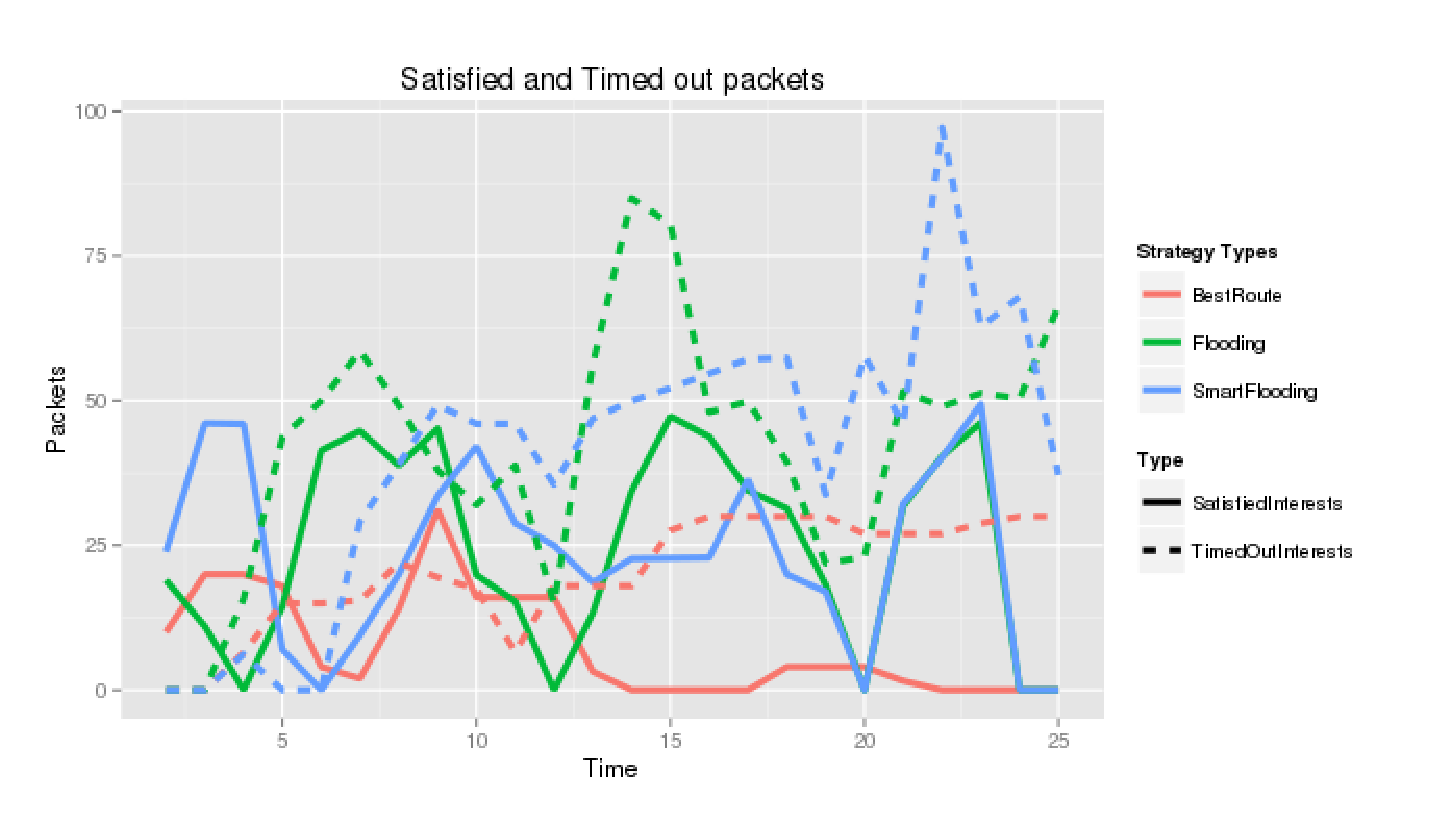
\epsfig{file=satisfied-timeout.eps}}
%\caption{Network Satisfied and Timed Out Interest Packets over time}
%\label{fig:sattimeint}
%\end{figure}

Using table \ref{tab:packetsum}, we can notice that the amount of content
received in the ideal case is 214. For SmartFlooding this is just above half at
108.5 but below half for Flooding and BestRoute while having a substantial 
increase in satisfied and timed out interests, which point to more network 
traffic generation. 

It is important to point out that the strategies used do not attempt to find
the desired content beyond controlling for the number of timed out Interest
packets, which is it's only feedback mechanism. On a positive note, compared to
current networks, there is a high probability of obtaining some data, as the
Interest packets generated don't have particular destination addresses and are
only limited by their timeouts.

It is obvious that a basic ICN would be completely useless for any time and
jitter sensitive applications that require a mobile provider. 

We find it apparent that we require a mechanism in ICN to better our mobility,
particularly for mobile providers. What is not apparent is where this mechanism 
should be placed. As far as we know, Saltzer
\cite{saltzer:namingandbindingnetworks} and Day's guidelines
\cite{Day:2008:PNA:1349793} are not being followed because they suggest three 
sets of name spaces; PoAs, Nodes and Applications. This would also require 2 name
space resolution mechanisms to pass from one name space to another. This would
go directly against the core of ICN specifications. Thus it would seem that we
require methods to augment the knowledge of the network state in every
particular ICN router to improve forwarding.

\section{Conclusion}
We have proposed a code base with a topology and metrics to assess ICN mobility
proposals. With our proposal we have demonstrated the lack of support for
provider mobility in ICN and have set a basic metric with which to compare other
proposals. We also briefly discussed issues regarding naming in networks for 
mobility.

%\section*{Acknowledgement}
%This research was supported by a grant-in-aid from the High-Tech Research
%Center Project of the Ministry of Education, Culture, Sports, Science and
%Technology (MEXT) \cite{mext:2014:Online}, Japan.

\bibliographystyle{acm}
\bibliography{myrefs}

\end{document}
